%%%%%%%%%%%%%%%%%%%%%%%%%%%%%%%%%%%%%%%%%%%%%%%%%%%%%%%%%%%%%%%%%%%%%%%%%%
%%%%%                         CHAPITRE 6                            %%%%%%
%%%%%%%%%%%%%%%%%%%%%%%%%%%%%%%%%%%%%%%%%%%%%%%%%%%%%%%%%%%%%%%%%%%%%%%%%%

\lhead[\fancyplain{}{\leftmark}]%Pour les pages paires \bfseries
      {\fancyplain{}{}} %Pour les pages impaires
\chead[\fancyplain{}{}]%
      {\fancyplain{}{}}
\rhead[\fancyplain{}{}]%Pour les pages paires 
      {\fancyplain{}{\rightmark}}%Pour les pages impaires \bfseries
\lfoot[\fancyplain{}{}]%
      {\fancyplain{}{}}
\cfoot[\fancyplain{}{\thepage}]%\bfseries
      {\fancyplain{}{\thepage}} %\bfseries
\rfoot[\fancyplain{}{}]%
     {\fancyplain{}{\scriptsize}}


%%%%%%%%%%%%%%%%%%%%%%%%%%%%%%%%%%%%%%%%%%%%%%%%%%%%%%%%%%%%%%%%%%%%%%%%%%
%%%%%                      Start part here                          %%%%%%
%%%%%%%%%%%%%%%%%%%%%%%%%%%%%%%%%%%%%%%%%%%%%%%%%%%%%%%%%%%%%%%%%%%%%%%%%%

\chapter{Application to boxing, using action cameras}
\label{ch:6}

%%% TITRE ARTICLE
%%% Evaluation of kinematic performance indicators in boxing in suboptimal conditions
%%% TITRE



%==============================================================================	Résumé du chapitre

\begin{center}
\rule{0.7\linewidth}{.5pt}
\begin{minipage}{0.7\linewidth}
\smallskip

\textit{Boxing is a challenging sport for motion analysis, because movements are fast, 3 dimensional, and involve the whole body. Moreover, it is usually not possible to equip a boxer with markers, lightning conditions and large capture volumes make the classic marker-based difficult, research-grade cameras are too cumbersome to set up in a timely way and lower-end cameras can't be synchronized by hardware, nor with a flash in the context of a competition.\newline\newline
The objective of the study was to verify whether it is possible to accurately measure Key Performance Indicators (KPIs) in boxing, with a markerless protocol and under suboptimal conditions. This was concurrently validated with a marker-based protocol. A secondary goal was to compare the impact on result quality of a markerless analysis with post-calibration and post-synchronization, to the impact of choosing a different 2D pose estimation model. We conclude that KPIs are remarkably well evaluated in all conditions, although the choice of the 2D pose estimator is more influential than the protocol. \newline \newline
This chapter is adapted from the poster presented at the congress of the European College of Sport Science (ECSS): "A 3D markerless protocol with action cameras – Key performance indicators in boxing" \cite{Pagnon2022c}.
}

%\smallskip
\end{minipage}
\smallskip
\rule{0.7\linewidth}{.5pt}
\end{center}

\clearpage

\minitoc

\vspace*{3cm}

\begin{figure}[hbtp]
	\centering
	\def\svgwidth{1\columnwidth}
	\fontsize{10pt}{10pt}\selectfont
	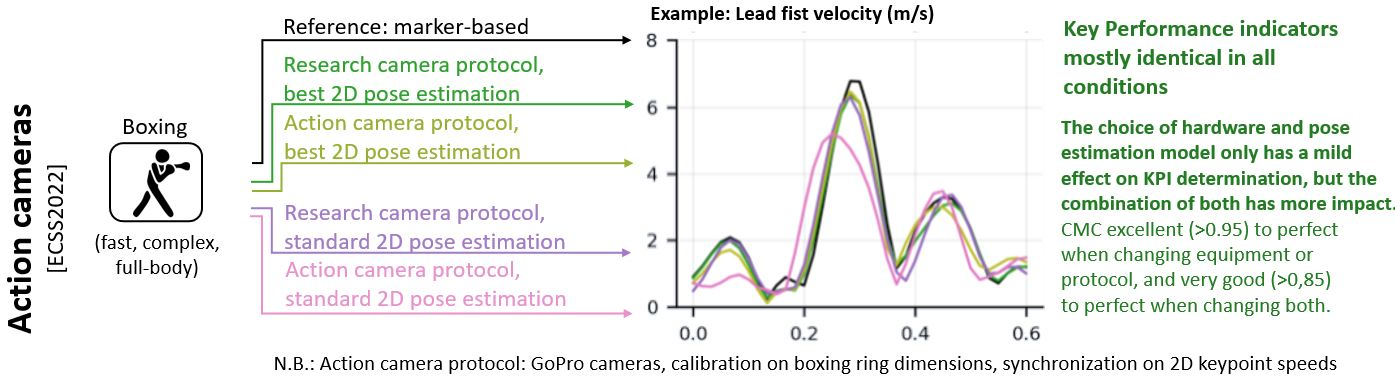
\includegraphics[width=\linewidth]{"../Intro/Figures/Fig_VisAbstract4.JPG"}
      \caption{Visual abstract for the assessment of KPIs in boxing with Pose2Sim \cite{Pagnon2022c}.}
	\label{fig_visabstract4}
\end{figure}

\newpage






\section{Introduction}

\subsection{Key Performance Indicators in boxing}

Key Performance Indicators (KPIs) are a set of variables which need to be measured in priority, in order to assess performance, or to evaluate main areas where work is needed. Although they are more known in the fields of management or of the industry, identifying them is also important in sports \cite{Hughes2002,Butterworth2013}. Determining them would typically be done in two steps. First, through discussions with coaches, who usually have a subjective, but nevertheless very fine and comprehensive understanding of their sport. Then, the most relevant of these variables can be selected, for example by Principal Component Analysis (PCA) \cite{Hotelling1933}. PCA allows for grouping the variables that explain most of the performance, and excluding the others \cite{ODonoghue2008}.

However, this approach has the disadvantage that prior to pursuing any further statistical analysis, all the potential variables first need to be extensively recorded. Only then, the most relevant ones can be determined. Moreover, it might lead to the selection of indicators which can be hard to retrieve, or be not intuitively meaningful as they potentially consist in the linear combination of some seemingly unrelated variables. In this case, one can choose the performance indicator most associated with each principal component \cite{ODonoghue2008}. Other methods exist, such as exclusive expert coach opinion, hierarchical models based on breaking down individual techniques, or notational analysis based on scoring events and actions along a competition, or other inferential statistics such as regression analysis, and more \cite{Hughes2002,Butterworth2013}.

KPIs in boxing can be separated into several categories: action annotations (such as points scored, number of recorder jabs punches or dodging by leaning backwards \cite{Thomson2013}), anthropometric KPIs (such as long arm length and high muscle percentage \cite{Chaabene2015}), physiological (such as high velocity at maximal oxygen uptake and high anaerobic power \cite{Chaabene2015}), or biomechanical (such as ground reaction force of the rear leg before execution of a cross punch, activation of the latissiums dorsi during the hook punch, or extension of the elbow at the end of the execution of the jab \cite{Lenetsky2020}). 

Among all these KPIs, we focus on a subset of the biomechanic ones, namely kinematics. Ultimately, a decisive aspect in a punch is its speed, which determines how powerful it is (along with force), and how difficult it will be for the opponent to dodge it. However, speed is not generated the same way in jabs as in hooks, since one is a mostly translational movement whereas the other is mostly rotational. \cite{Lenetsky2020} broke down the phases of both techniques. Among other body motions, the jab involves translating the lead foot toward the target, then the pelvis and the torso follow, while the lead arm flexes at the elbow to store elastic energy prior to throwing the punch. Finally, the elbow extends, until the fist is brought into contact with the target. Regarding the rear hook, it starts with flexion of the rear knee, while the pelvis and torso rotate horizontally away from the target. Then the motion is reversed, as the knee extends and the pelvis and torso rotate toward the target. Lastly, the attacking arm abducts at the shoulder until the fist reaches the target. 

As a consequence, it seems like the lead foot translation, the pelvis translation, the lead elbow extension, and the lead fist velocity would consist in good KPIs for the jab, and the rear knee flexion, the pelvis rotation, the rear shoulder extension, and the rear fist velocity would be valuable to estimate for the rear hook.


\subsection{Limits of research-grade systems in competitions}

When fine kinematic analysis is needed, the de facto method is marker-based motion capture. However, it is not appropriate in sports, as it involves laying markers directly on the skin, which is not conceivable during a match or a sparring session. It is intrusive and cumbersome, and usually involves specific environment conditions. Moreover, markers can fall off the body when the athlete is sweating or moving fast. As a consequence, it is important to investigate markerless techniques. 

Another constraint of sports analysis is the capture system, which needs to be discrete and installed swiftly. As a consequence, research grade video systems such as Qualisys are not appropriate: they involve setting up large cameras and stands, with cumbersome power and synchronization cables, which are cumbersome and prevent cameras from being spread too far apart. These systems require at least two trained operators to set them up and to adjust their parameters. They are also very expensive, while their framerate and resolution are not very good. On the other end, consumer-grade action cameras such as GoPros are very small, don't necessitate any cabling, and the operator has nothing to do but clicking the recording button. They are also cheap, and offer remarkably high framerate, resolution, and image quality. However, their battery does not last more than an hour, they don't come with calibration, and until recently, no synchronization solution existed. There is also no centralized visual feedback on the recording.

When outdoors, in direct sunlight and with large capture volumes, extrinsic calibration of video cameras with markers becomes very delicate, too. Markers are inconstantly detected, and no reliable solution currently exists, including with active LED markers. Checkerboard calibration is almost equally problematic, as corners are not always well detected unless it is too large to conveniently carry around. Other solutions exist, such as calibrating intrinsic parameters with a checkerboard, and extrinsic parameters with manually clicked and semi-automatically tracked points on a wand \cite{Argus2017}. Alternatively, it is possible to calibrate extrinsics on any object of known dimensions \cite{Dawson-Howe1994}, be it a human being \cite{Liu2022a}.

Lastly, synchronization can also be a problem. Using a trigger signal is the most accurate method, but again, it generally involves using wired cameras. Other methods rely on using a flash, or an audio clap, but they are not possible in the context of a competition. Moreover, the speed of sound is not instantaneous, and the synchronization will not be very accurate on a large capture space if the distance from cameras to sound source is not taken into account \cite{Hasler2009}. For example, a 20 meters difference would lead to a 60 ms shift, which represents 7 frames at 120 fps. Other procedures can be explored, such as WiFi synchronization \cite{Romanov2019} or Bluetooth synchronization \cite{Asgarian2022}, but they usually require using external devices. GPS synchronization is compatible with GoPro 9 and plus, but it has not been evaluated yet \cite{GoPro2022}. Another way to synchronize is to cross-correlate different data streams, and to infer the delay between them from the time of maximum correlation \cite{Plotz2012}. 


\subsection{Objectives}

Evaluating kinematic KPIs in boxing is challenging both with marker-based and markerless techniques, mainly because movements are fast, 3 dimensional, and whole body. Moreover, addressing motion capture in sports leads to constraints on the protocol, and involve carefully thinking about the hardware, about the calibration method, and about the synchronization procedure. These three elements determine 3D reconstruction. However, before this stage comes the 2D pose estimation. 

Numerous solutions exist in this regard. AlphaPose \cite{Fang2017} and OpenPose \cite{Cao2019} are the most common, and the most accurate \cite{Needham2021b,Mroz2021}. OpenPose is even more widely used than AlphaPose, which is why we will focus on this human pose detector. Its standard model is body\_25, however the body\_25B subset of the single-network whole-body pose estimation \cite{Hidalgo2019} also provides 25 points, is as fast as the standard one, and is claimed to be more accurate and to reduce false positives \cite{Hidalgo2019,Pagnon2021}. 

The objective of this study is to evaluate how accurately KPIs are retrieved in suboptimal conditions. We will analyze the impact of choosing a markerless protocol, with lower-end cameras, post-calibration on the boxing ring dimensions, post-synchronization on cross-correlation of 2D keypoint speeds, and a standard but less accurate 2D pose estimation model.



Subject not well detected?

Markers, Cameras et setup, Calibration, synchronization, Feedback


shadow boxing


\cite{Haralabidis2020} monitored the effect of fatigue on punching performance by fusing the outputs of IMUs with those of OpenPose processed videos. However, is this is not a full markerless protocol, we opt for performing kinematic analysis with Pose2Sim \cite{Pagnon2022b} (see \autoref{ch:3}).

Concurrently validating the accuracy of KPI measurements in boxing with suboptimal markerless protocols.


\section{Methods}
\subsection{4 conditions}
\blindtext

\subsection{Pose-calibration on ring dimensions}
\blindtext

\subsection{Post-synchronization on 2D movement speeds}
\blindtext

\subsection{GoPro spatio-temporal base into Qualysis'}
\blindtext

\subsection{Statistical analysis}
\blindtext


\section{Results}
\blindtext


\section{Discussion}
\subsection{Equipment and protocol vs. pose estimation model}

We evaluated that the 3D reconstruction could work reliably in most conditions, and that with the current state of the art, carefully choosing a good 2D pose estimation model was more important. However, kinematics from video cameras involve 3 main stages: 2D pose estimation, 3D reconstruction, and kinematic optimization. The last one has not been evaluated, and yet, it is of crucial importance. Choosing a good kinematic model with consistent constraints and bone definitions will determine whether the results can be trusted, or not. In particular, in this study the shoulder was defined as a ball joint, both on the marker-based and on the markerless analysis. However, the scapulothoracic girdle is a very complex multi-articulated joint, which allows for 3 rotations and 3 translations \cite{Seth2016}. Considering how little keypoints are tracked by the standard 3D pose estimators, it is impossble to use a more complex model. However, our shoulder abduction results can probably not be entirely trusted, neither for our markerless nor for our marker-based protocol (see \nameref{ch3_lim} in \autoref{ch:3}).

% Calibration remains a challenging task in daylight, at a distance, with non research-grade cameras, and in a sports scene. It could be useful to make it more robust, either by implementing the Aniposelib library \cite{Karashchuk2020}, or by calibrating automatically on people’s limb length \cite{Liu2022a}.



% Adding muscles which were stripped from the skeleton in the OpenSim model could allow for joint kinetics prediction. Neural networks could be trained to estimate ground reaction forces from kinetics on specific tasks, without the use of a force platform [Oh2013, Johnson2018, Mundt2019].
% Using Xsens markers hidden by clothes in Kinovis? Although not gold-standard


\subsection{Pros and cons of different systems}

Auto-calibration with person?

Cloud computing?

Temporal consistency?

Shape information for less cameras?

Rolling shutter: Pour les GoPros, la fréquence de roll du shutter de haut en bas est approxivement la même que la fréquence d'acquisition, donc vu qu'on peut filmer jusqu'à 240 Hz en full HD, 120Hz en 4K, et 60Hz à 5.3k, je doute que ce soit un vrai problème...
Pas de retour visuel instantanné
Synchro : nouvelles avec GPS, sinon méthodes
Calib : Mieux qu'avec Qualisys en plein air

